% 000.main_ijac.tex
% Template LaTeX - Iberoamerican Journal of Applied Computing (IJAC)
% ISSN 2237-4523

\documentclass[11pt,a4paper]{article}
\usepackage{url}
% =========================================================
% LANGUAGE AND ENCODING
% =========================================================
\usepackage[utf8]{inputenc}
\usepackage[T1]{fontenc}
\usepackage[english]{babel} % Ajustado para english devido ao conteúdo dos arquivos

% =========================================================
% PAGE CONFIGURATION
% =========================================================
\usepackage[
    a4paper,
    left=2.5cm,
    right=2.5cm,
    top=3.0cm,
    bottom=3.0cm
]{geometry}

\usepackage{setspace}
\usepackage{ragged2e}
\usepackage{times}
\usepackage{indentfirst}

\setlength{\parindent}{1.25cm}
\setlength{\parskip}{0pt}

% =========================================================
% COLORS
% =========================================================
\usepackage{xcolor}

\definecolor{ijacmaroon}{RGB}{115,20,40}

% =========================================================
% DADOS DO ARTIGO (Variáveis)
% =========================================================
% 001.basicdata.tex
% Variáveis com os dados do artigo para injeção no template da IJAC

% 1. Título do Artigo
\newcommand{\ijactitle}{Example File for Articles adapted for IJAC}

% 2. Autores (utilize $^1$, $^2$ etc para associar às instituições)
\newcommand{\ijacauthors}{Author Name 1$^1$, Author Name 2$^1$, Author Name 3$^2$}

% 3. Instituições / Endereços
\newcommand{\ijacaddress}{
  $^1$Graduate Program -- University XXX -- City -- State -- Country\\
  $^2$Department Name -- Another Institution (ACRONYM) -- City -- State -- Country
}

% 4. E-mails
\newcommand{\ijacemails}{\texttt{test1@uni.br, test2@uni.br, test3@uni.br}}

% 5. Informações de Rodapé para a IJAC (Volume, Número, Ano, etc.)
\newcommand{\ijacvolume}{Vol. 10, No. 2}
\newcommand{\ijacano}{2026}


% =========================================================
% HEADER AND FOOTER
% =========================================================
\usepackage{fancyhdr}

\setlength{\headheight}{14pt}

\pagestyle{fancy}
\fancyhf{}

\renewcommand{\headrulewidth}{0pt}
\renewcommand{\footrulewidth}{0pt}

\fancyhead[L]{%
    \color{ijacmaroon}
    \bfseries\itshape\small
    Iberoamerican Journal of Applied Computing
}

\fancyhead[R]{%
    \color{ijacmaroon}
    \bfseries\itshape\small
    ISSN 2237-4523
}

\fancyfoot[L]{%
    \color{ijacmaroon}
    \bfseries\itshape
    \ijacvolume, \ijacano
}

\fancyfoot[R]{%
    \color{ijacmaroon}
    \bfseries\itshape
    Page \thepage
}

% =========================================================
% HEADER AND FOOTER LINES
% =========================================================
\usepackage{tikz}
\usetikzlibrary{calc}

\AddToHook{shipout/background}{%
    \begin{tikzpicture}[remember picture,overlay]

        \draw[
            ijacmaroon,
            line width=1.4pt
        ]
        ($(current page.north west)+(2.5cm,-2.35cm)$)
        --
        ($(current page.north east)+(-2.5cm,-2.35cm)$);

        \draw[
            ijacmaroon,
            line width=1.4pt
        ]
        ($(current page.south west)+(2.5cm,2.3cm)$)
        --
        ($(current page.south east)+(-2.5cm,2.3cm)$);

    \end{tikzpicture}%
}

% =========================================================
% SECTION TITLES
% =========================================================
\usepackage{titlesec}

\titleformat{\section}
    {\bfseries}
    {\thesection.}
    {0.5em}
    {}

\titleformat{\subsection}
    {\bfseries\itshape}
    {\thesubsection}
    {0.5em}
    {}

\titleformat{\subsubsection}
    {\bfseries}
    {\thesubsubsection}
    {0.5em}
    {}

\titlespacing*{\section}
    {0pt}
    {1.5em}
    {0.8em}

\titlespacing*{\subsection}
    {0pt}
    {1.2em}
    {0.6em}

\titlespacing*{\subsubsection}
    {0pt}
    {1em}
    {0.5em}

% =========================================================
% FIGURES AND TABLES
% =========================================================
\usepackage{graphicx}
\usepackage{array}
\usepackage{booktabs}
\usepackage{float}
\usepackage{caption}

\captionsetup[figure]{
    labelsep=endash,
    justification=centering,
    font=small
}

\captionsetup[table]{
    labelsep=period,
    justification=centering,
    font=small,
    position=top
}

% =========================================================
% MATHEMATICS
% =========================================================
\usepackage{amsmath}
\usepackage{amssymb}

% =========================================================
% SOURCE CODE
% =========================================================
\usepackage{listings}

\renewcommand{\lstlistingname}{Code}
\renewcommand{\lstlistlistingname}{List of Codes}

\lstset{
    basicstyle=\ttfamily\footnotesize,
    breaklines=true,
    breakatwhitespace=false,
    frame=single,
    columns=fullflexible,
    keepspaces=true,
    showstringspaces=false,
    captionpos=b,
    numbers=none,
    tabsize=2,
    xleftmargin=0.5cm,
    xrightmargin=0.5cm,
    aboveskip=0.8em,
    belowskip=0.8em
}

% =========================================================
% HYPERLINKS (DEVE VIR ANTES DO ABNTEX2CITE)
% =========================================================
\usepackage{hyperref}

\hypersetup{
    colorlinks=true,
    linkcolor=black,
    citecolor=black,
    urlcolor=blue
}

% =========================================================
% REFERENCES CONFIG (DEVE VIR DEPOIS DO HYPERREF)
% =========================================================
\usepackage[
    alf,
    recuo=0cm,
    abnt-etal-text=it,
    bibjustif,
    abnt-emphasize=bf
]{abntex2/abntex2cite}

% =========================================================
% AMBIENTES DE RESUMO MODULARES
% =========================================================
\renewenvironment{abstract}{%
    \begin{quote}\itshape\noindent\textbf{Abstract.} 
}{%
    \end{quote}\vspace{0.5em}
}

\newenvironment{resumo}{%
    \begin{quote}\itshape\noindent\textbf{Resumo.} 
}{%
    \end{quote}\vspace{1.0em}
}

% =========================================================
% DOCUMENT
% =========================================================

\begin{document}

\begin{center}
  {\large\bfseries \ijactitle}
  \vspace{0.8em}

  {\bfseries \ijacauthors}
  \vspace{0.6em}

  \ijacaddress
  \vspace{0.3em}

  \ijacemails
\end{center}

\vspace{1.2em}

% Inclusão dos conteúdos externos
\begin{abstract}
  This is a dummy abstract. It describes the style to be used in articles and short papers for the IJAC journal. Abstracts should not have more than 10 lines and must be in the first page of the paper.
\end{abstract}
\section{Introduction}
This file serves only as a reading and testing base. 

It is configured to be executed one directory level above the abntex2 folder, requiring the package and bibliography calls to specify the relative path.

An example of a citation: \cite{knuth84}

For the bibliographic reference to work, remember to compile using BibTeX.

\section{Literature Review}
This area is reserved for the literature review. 

This is an example of a line break.

An example of an image, in Figure \ref{fig:example_ijac}.

\begin{figure}[ht]
\centering
% Updated to the IJAC folder and file
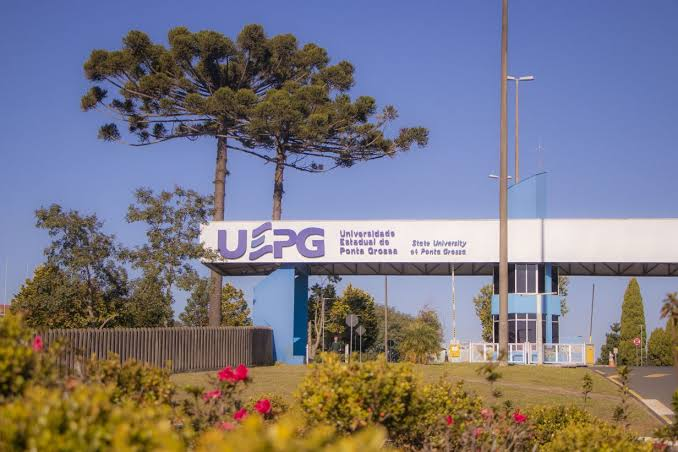
\includegraphics[width=0.5\textwidth]{figures/fig1.jpeg}
\caption{Just an example of a figure.}
\label{fig:example_ijac}
\end{figure}

\section{Material and Methods}
Area for description of material and methods. Table \ref{tab:example_methods} presents an example of a table.

\begin{table}[ht]
\centering
\caption{An example of a table}
\label{tab:example_methods}
\begin{tabular}{lcc}
\hline
\textbf{Column number 1} & \textbf{Column 2} & \textbf{Column 3} \\
\hline
Row 2 Column 1& 6.02 & 7.01 \\
Row 3 Column 1 & 6.29 & 12.22 \\
Row 4 Column 1 & 4.66 & 3.47 \\
Row 5 Column 1 & 5.71 & 5.37 \\
\hline
\end{tabular}
\end{table}

\section{Results and Discussion}
This area is reserved for the presentation and discussion of the results.

\subsection{A subsection test}
Adding a subsection here. Below, an example of a formula:

\begin{equation}
P(A|B) = \frac{P(B|A)P(A)}{P(B)}
\label{eq:bayes}
\end{equation}

\subsection{Another subsection}
Now, showing items:

\begin{itemize}
    \item Item 1;
    \item Item 2;
    \item Item 3.
\end{itemize}

\subsection{Presentation of Algorithms and Code}
When it is strictly necessary to demonstrate the inference logic or feature extraction without resorting to formal pseudocode.

\begin{lstlisting}[language=Python, breaklines=true, basicstyle=\ttfamily\footnotesize]
def calc_prob(var1, var2):
    
    if var1 > var2:
        return "Var1 is greater than Var2"
    return "Var1 is less than or equal to Var2"
\end{lstlisting}

\section{Conclusion}
Finally, the conclusion.


% =========================================================
% REFERENCES
% =========================================================
\bibliographystyle{abntex2/abntex2-alf}
\bibliography{200.referencesjabref}

\end{document}
